
\documentclass[9pt]{beamer}
%\makeatletter
%\def\beamer@calltheme#1#2#3{%
%	\def\beamer@themelist{#2}
%	\@for\beamer@themename:=\beamer@themelist\do
%	{\usepackage[{#1}]{\beamer@themelocation/#3\beamer@themename}}}
%
%\def\usefolder#1{
%	\def\beamer@themelocation{#1}
%}
%\def\beamer@themelocation{}

%\usefolder{../config}

\usetheme[
block=fill,
titleformat=regular,
progressbar=frametitle
]{metropolis}
%\metroset[everytitleformat=regular] % regular, lowercase, uppercase ]
%\metroset[inner/block=fill]

%\setbeameroption{show notes} 
\usepackage{booktabs}
\usepackage[scale=2]{ccicons}

\usepackage{pgfplots}
\usepgfplotslibrary{dateplot}


%\ Hrvatski znakovi
\usepackage[utf8]{inputenc}
\usepackage[T1]{fontenc}
\usepackage[croatian]{babel}
\usepackage{todonotes}
\usepackage{amsmath}
\usepackage{amsfonts}
\selectlanguage{croatian} % american ngerman
\usepackage{todonotes}

% Koristenje Latin modern fonta
% Bez toga na nekim racunalima baca
% err: Font <taj i taj> at <mala velicina, npr4.0pt> not loadable: Metric (TFM) file not found. \end{frame}
\usepackage{lmodern}


\definecolor{RoyalBlue}{cmyk}{1, 0.50, 0, 0}
%\usepackage{natbib}
%\usepackage{bibentry}
\usepackage{scrextend}
\usepackage{hyperref}
%\usepackage[pdfa=true]{hyperref}
\hypersetup{%
    %draft, % = no hyperlinking at all (useful in b/w printouts)
    %colorlinks=true, 
    linktocpage=true, pdfstartpage=3, pdfstartview=FitV,%
    % uncomment the following line if you want to have black links (e.g., for printing)
    %colorlinks=false, linktocpage=false, pdfborder={0 0 0}, pdfstartpage=3, pdfstartview=FitV,% 
    breaklinks=true, pdfpagemode=UseNone, pageanchor=true, pdfpagemode=UseOutlines,%
    plainpages=false, bookmarksnumbered, bookmarksopen=true, bookmarksopenlevel=1,%
    hypertexnames=true, pdfhighlight=/O,%nesting=true,%frenchlinks,%
    %urlcolor=webbrown, linkcolor=RoyalBlue, citecolor=webgreen, %pagecolor=RoyalBlue,%
    %urlcolor=Blue, linkcolor=Blue, citecolor=Red, %pagecolor=Black,%
    %pdftitle={\myTitle},%
    %pdfauthor={\textcopyright\ \myName, \myUni, \myFaculty},%
    pdfsubject={},%
    pdfkeywords={},%
    pdfcreator={pdfLaTeX},%
    pdfproducer={LaTeX with hyperref and classicthesis}, %
    unicode = true 
} 

%\usepackage[pdftex]{graphicx}
% declare the path(s) where your graphic files are
\graphicspath{{./}{./figures/}}


\newcommand{\executeiffilenewer}[3]{%
	\ifnum\pdfstrcmp{\pdffilemoddate{#1}}%
	{\pdffilemoddate{#2}}>0%
	{\immediate\write18{#3}}\fi%
}
\newcommand{\includesvg}[1]{%
	\executeiffilenewer{#1.svg}{#1.pdf}%
	{inkscape -z -C --file=#1.svg %
		--export-pdf=#1.pdf --export-latex}%
	\input{#1.pdf_tex}%
}


% http://tex.stackexchange.com/questions/83882/how-to-highlight-python-syntax-in-latex-listings-lstinputlistings-command

\usepackage{listings}
\usepackage{color}
\usepackage[semibold]{sourcecodepro}

% Default fixed font does not support bold face
\DeclareFixedFont{\ttb}{T1}{txtt}{bx}{n}{12} % for bold
\DeclareFixedFont{\ttm}{T1}{txtt}{m}{n}{12}  % for normal
% Custom colors
\definecolor{deepblue}{rgb}{0,0,0.5}
\definecolor{deepred}{rgb}{0.6,0,0}
\definecolor{deepgreen}{rgb}{0,0.5,0}


% Python style for highlighting
\newcommand\pythonstyle{\lstset{
		language=Python,
		basicstyle=\small\ttfamily,
		otherkeywords={self},             % Add keywords here
		keywordstyle=\small\ttfamily\color{deepblue},
		emph={MyClass,__init__},          % Custom highlighting
		emphstyle=\small\ttfamily\color{deepred},    % Custom highlighting style
		stringstyle=\color{deepgreen},
		frame=tb,                         % Any extra options here
		showstringspaces=false            % 
	}}
	
	
	% Python environment
	\lstnewenvironment{python}[1][]
	{
		\pythonstyle
		\lstset{#1}
	}
	{}
	
	% Python for external files
	\newcommand\pythonexternal[2][]{{
			\pythonstyle
			\lstinputlisting[#1]{#2}}}
	
	% Python for inline
	\newcommand\pythoninline[1]{{\pythonstyle\lstinline!#1!}}

% \includeonlyframes{current}

%\documentclass[ucs]{beamer}
%\usetheme[menuwidth={0.3\paperwidth}]{erlangen}
%\setbeamercovered{transparent=20} 

\usepackage{amsmath,amsfonts,amsthm,amssymb}
\usepackage{setspace}
\usepackage{Tabbing}
\usepackage{fancyhdr}
\usepackage{lastpage}
\usepackage{extramarks}
\usepackage{chngpage}
\usepackage{soul,color}
\usepackage{graphicx,float,wrapfig}
\usepackage{xcolor}
\usepackage[normalem]{ulem}
\usepackage{mathtools}

\definecolor{erlangenlyellow}{RGB}{123, 25, 121}
%\usepackage[utf8x]{inputenc}
%\usepackage{default}
%\usepackage[T1]{fontenc}

\usepackage{verbatim}
\usepackage{listings}


\usepackage{subcaption}
\usepackage{lmodern}

\title{Teksture i protočni sustav}

% \subtitle{ Yet, it doesn't seem so clear to me anymore…?}
\subtitle {And so it was told, and so I told myself}
\institute{Računalna grafika}


\begin{document}
\begin{frame}
 \titlepage
\end{frame}

%\begin{frame}{Sadržaj}
%  \tableofcontents
%  % You might wish to add the option [pausesections]
%\end{frame}
% \section{Uvod}
\section{Grafički protočni sustav}
\begin{frame}{Protočni sustav}
	\begin{center}
		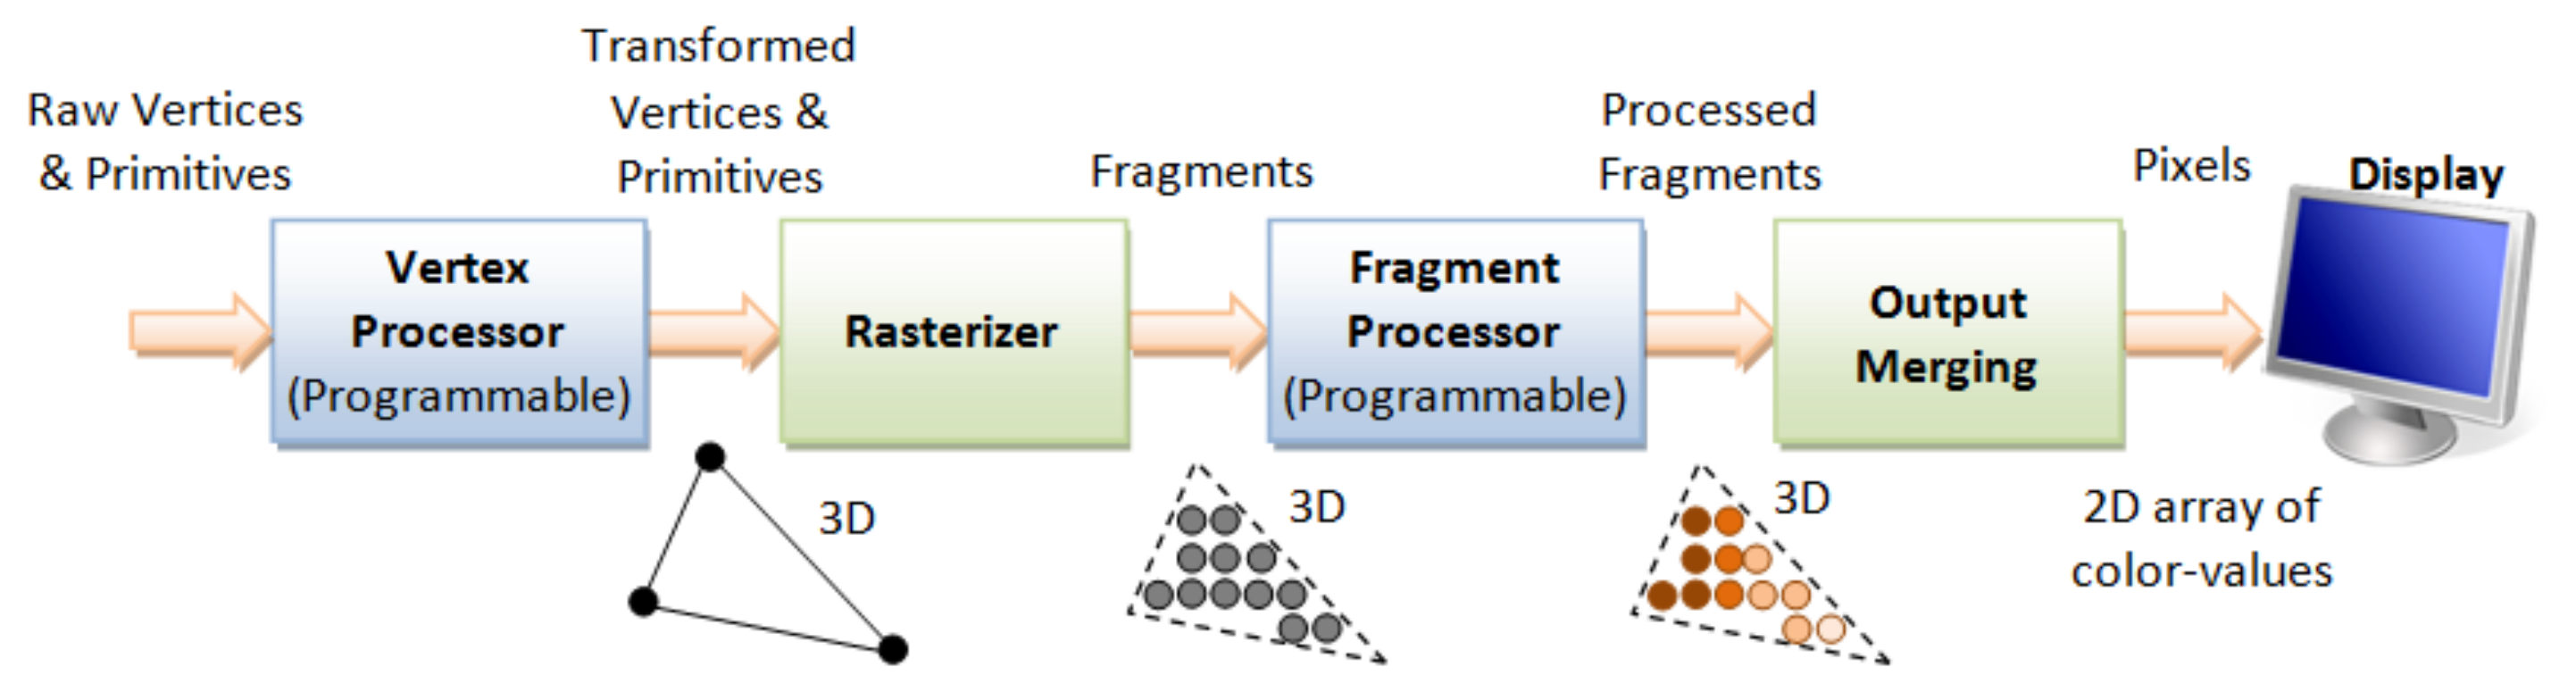
\includegraphics[width=10cm]{./slike/graphics_pipeline_01.png}
	\end{center}
\begin{itemize}
	\item Vertex Processing: Procesiranje i transformacija verteksa i normala
	\item Rasterizacija: Konverzija svakog primitiva (povezanih verteksa) u set fragmenata. Fragment, ugrubo: pikel s atributima (položaj, boja, normala i tekstura)
	\item Fragment Processing: Procesiranje fragmenata
	\item Output Merging: Spajanje fragmenata svih primitiva iz 3D u 2D color-pixel za prikaz
\end{itemize}
\end{frame}


\begin{frame}{Protočni sustav}
	\begin{center}
		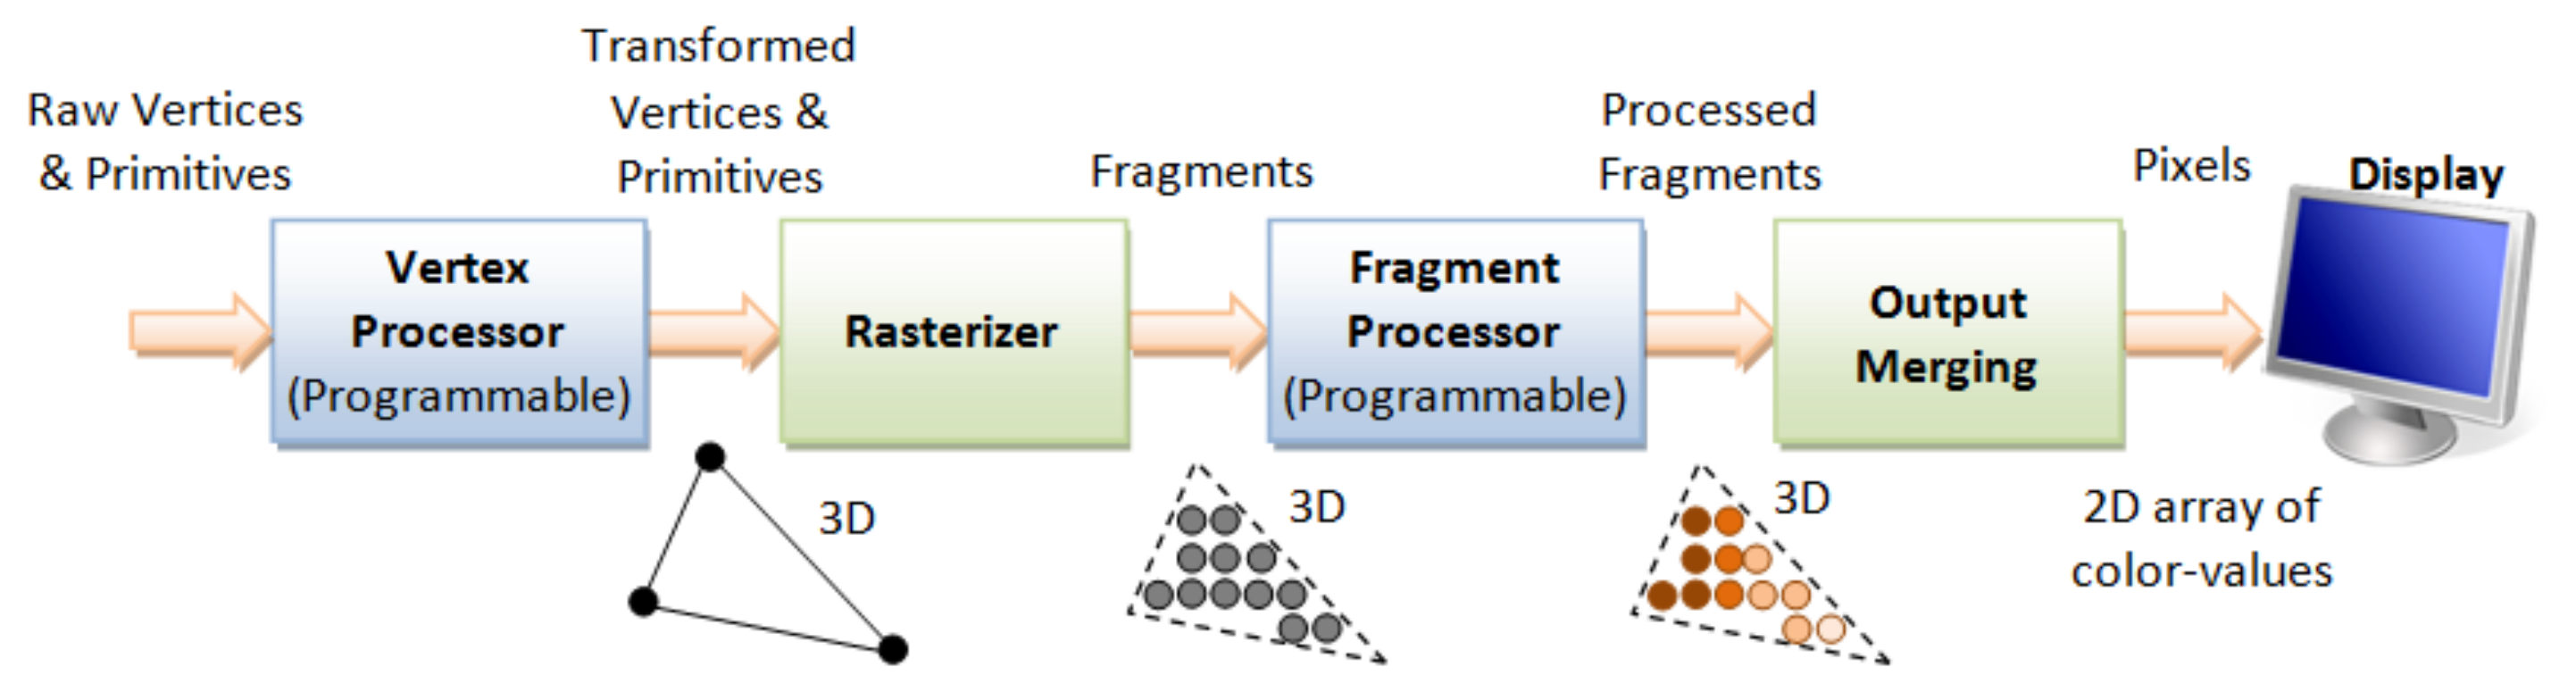
\includegraphics[width=10cm]{./slike/graphics_pipeline_01.png}
	\end{center}
	\begin{itemize}
		\item Vertex Processing: vertex shader: transformacije i osvjetljavanje za svaki verteks
		\item Fragment processor: fragment shader: teksture i osvjetljavanje za svaki fragment
	\end{itemize}
\end{frame}

\begin{frame}{Pixel vs fragment}
	\begin{center}
		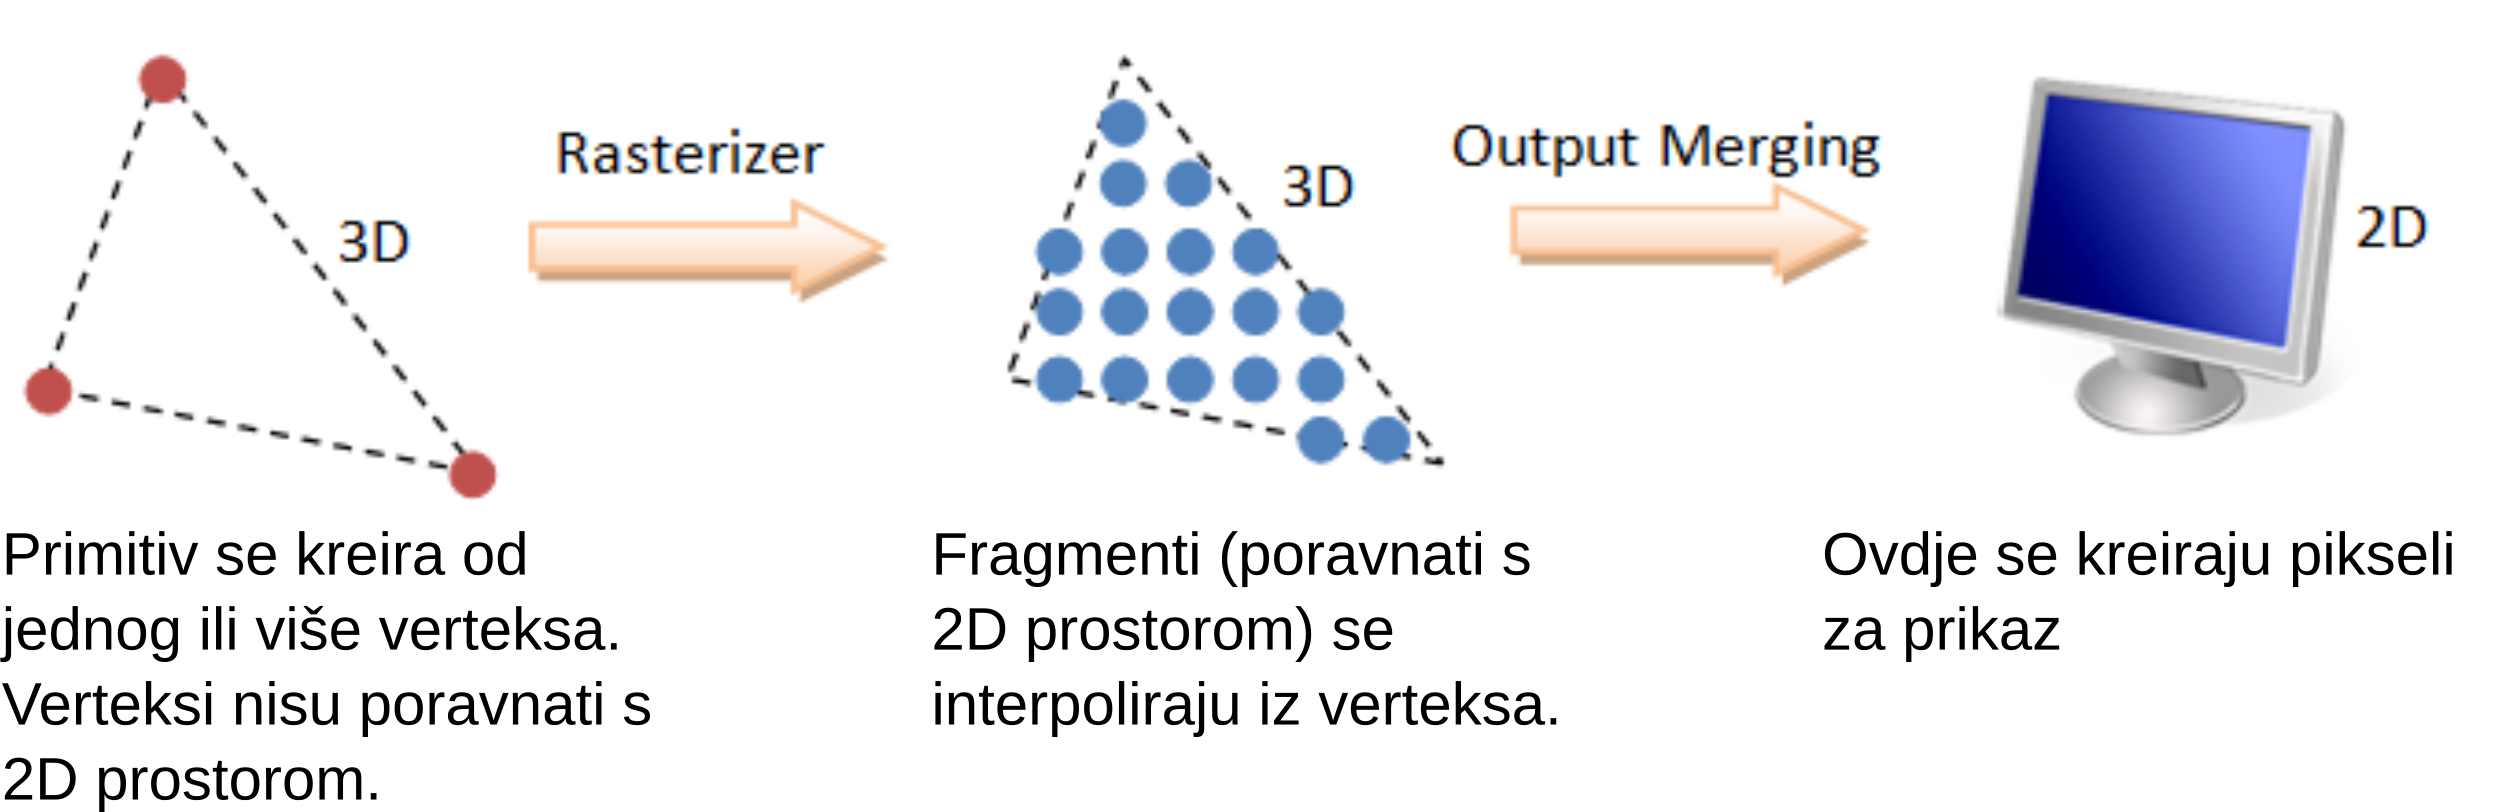
\includegraphics[width=6cm]{./slike/graphics_pipeline_02.png}
	\end{center}
\end{frame}

\begin{frame}{Protočni sustav}
	\begin{center}
		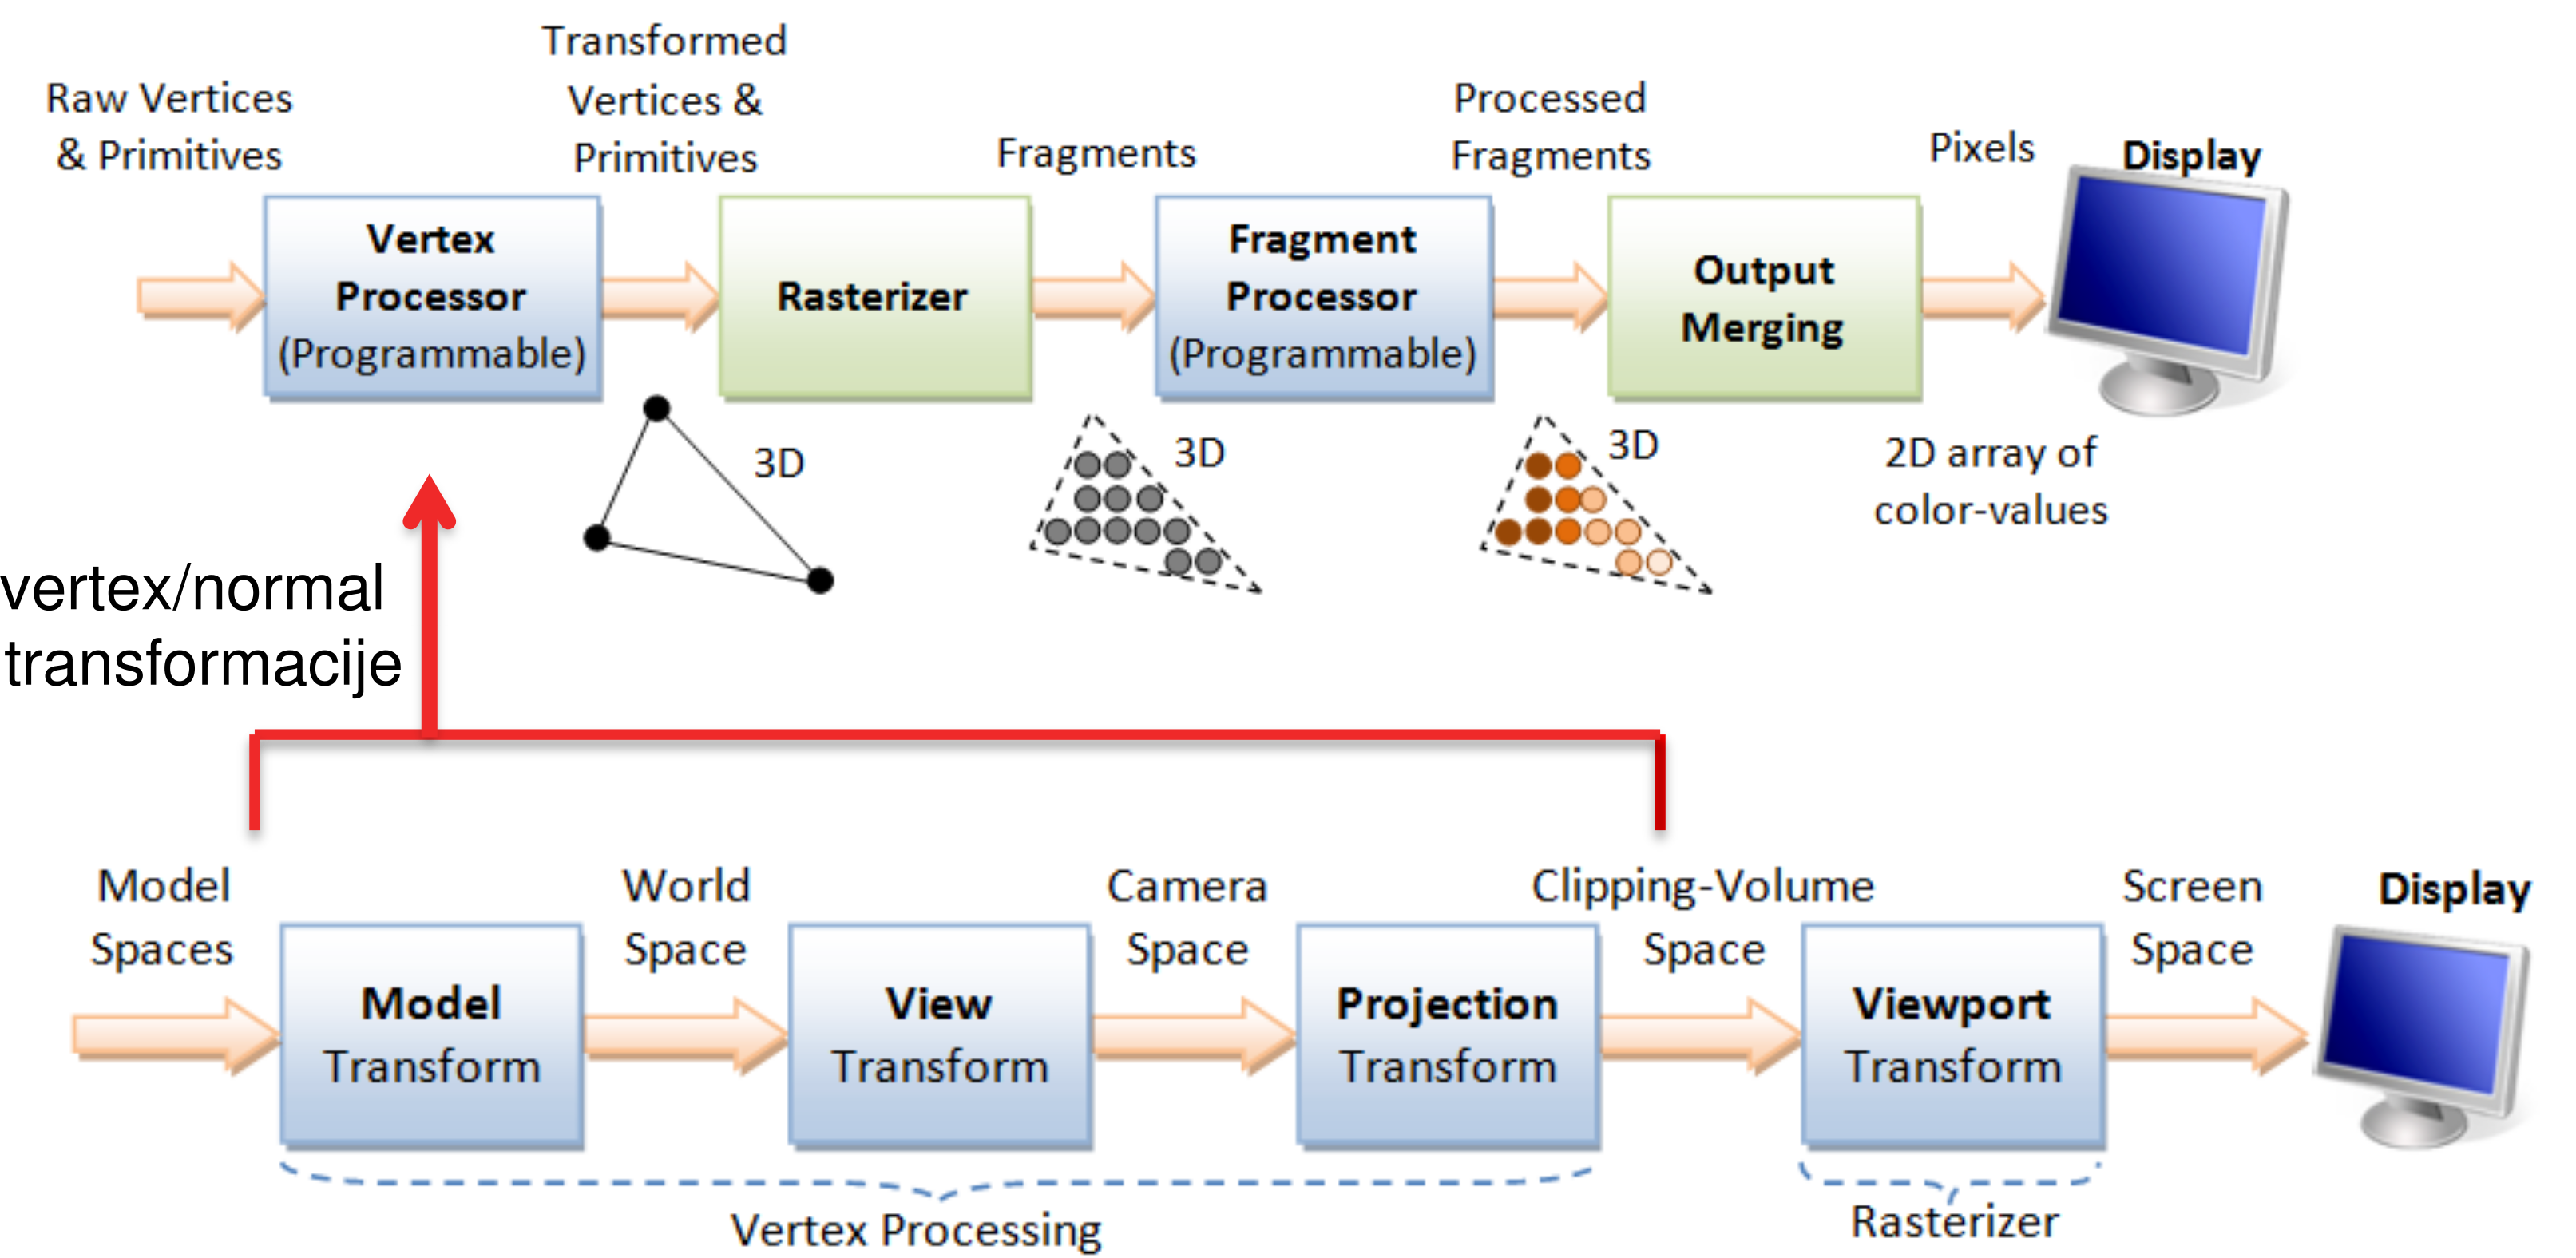
\includegraphics[width=10cm]{./slike/graphics_pipeline_03.png}
	\end{center}
\end{frame}

\begin{frame}{Protočni sustav}
	\begin{center}
		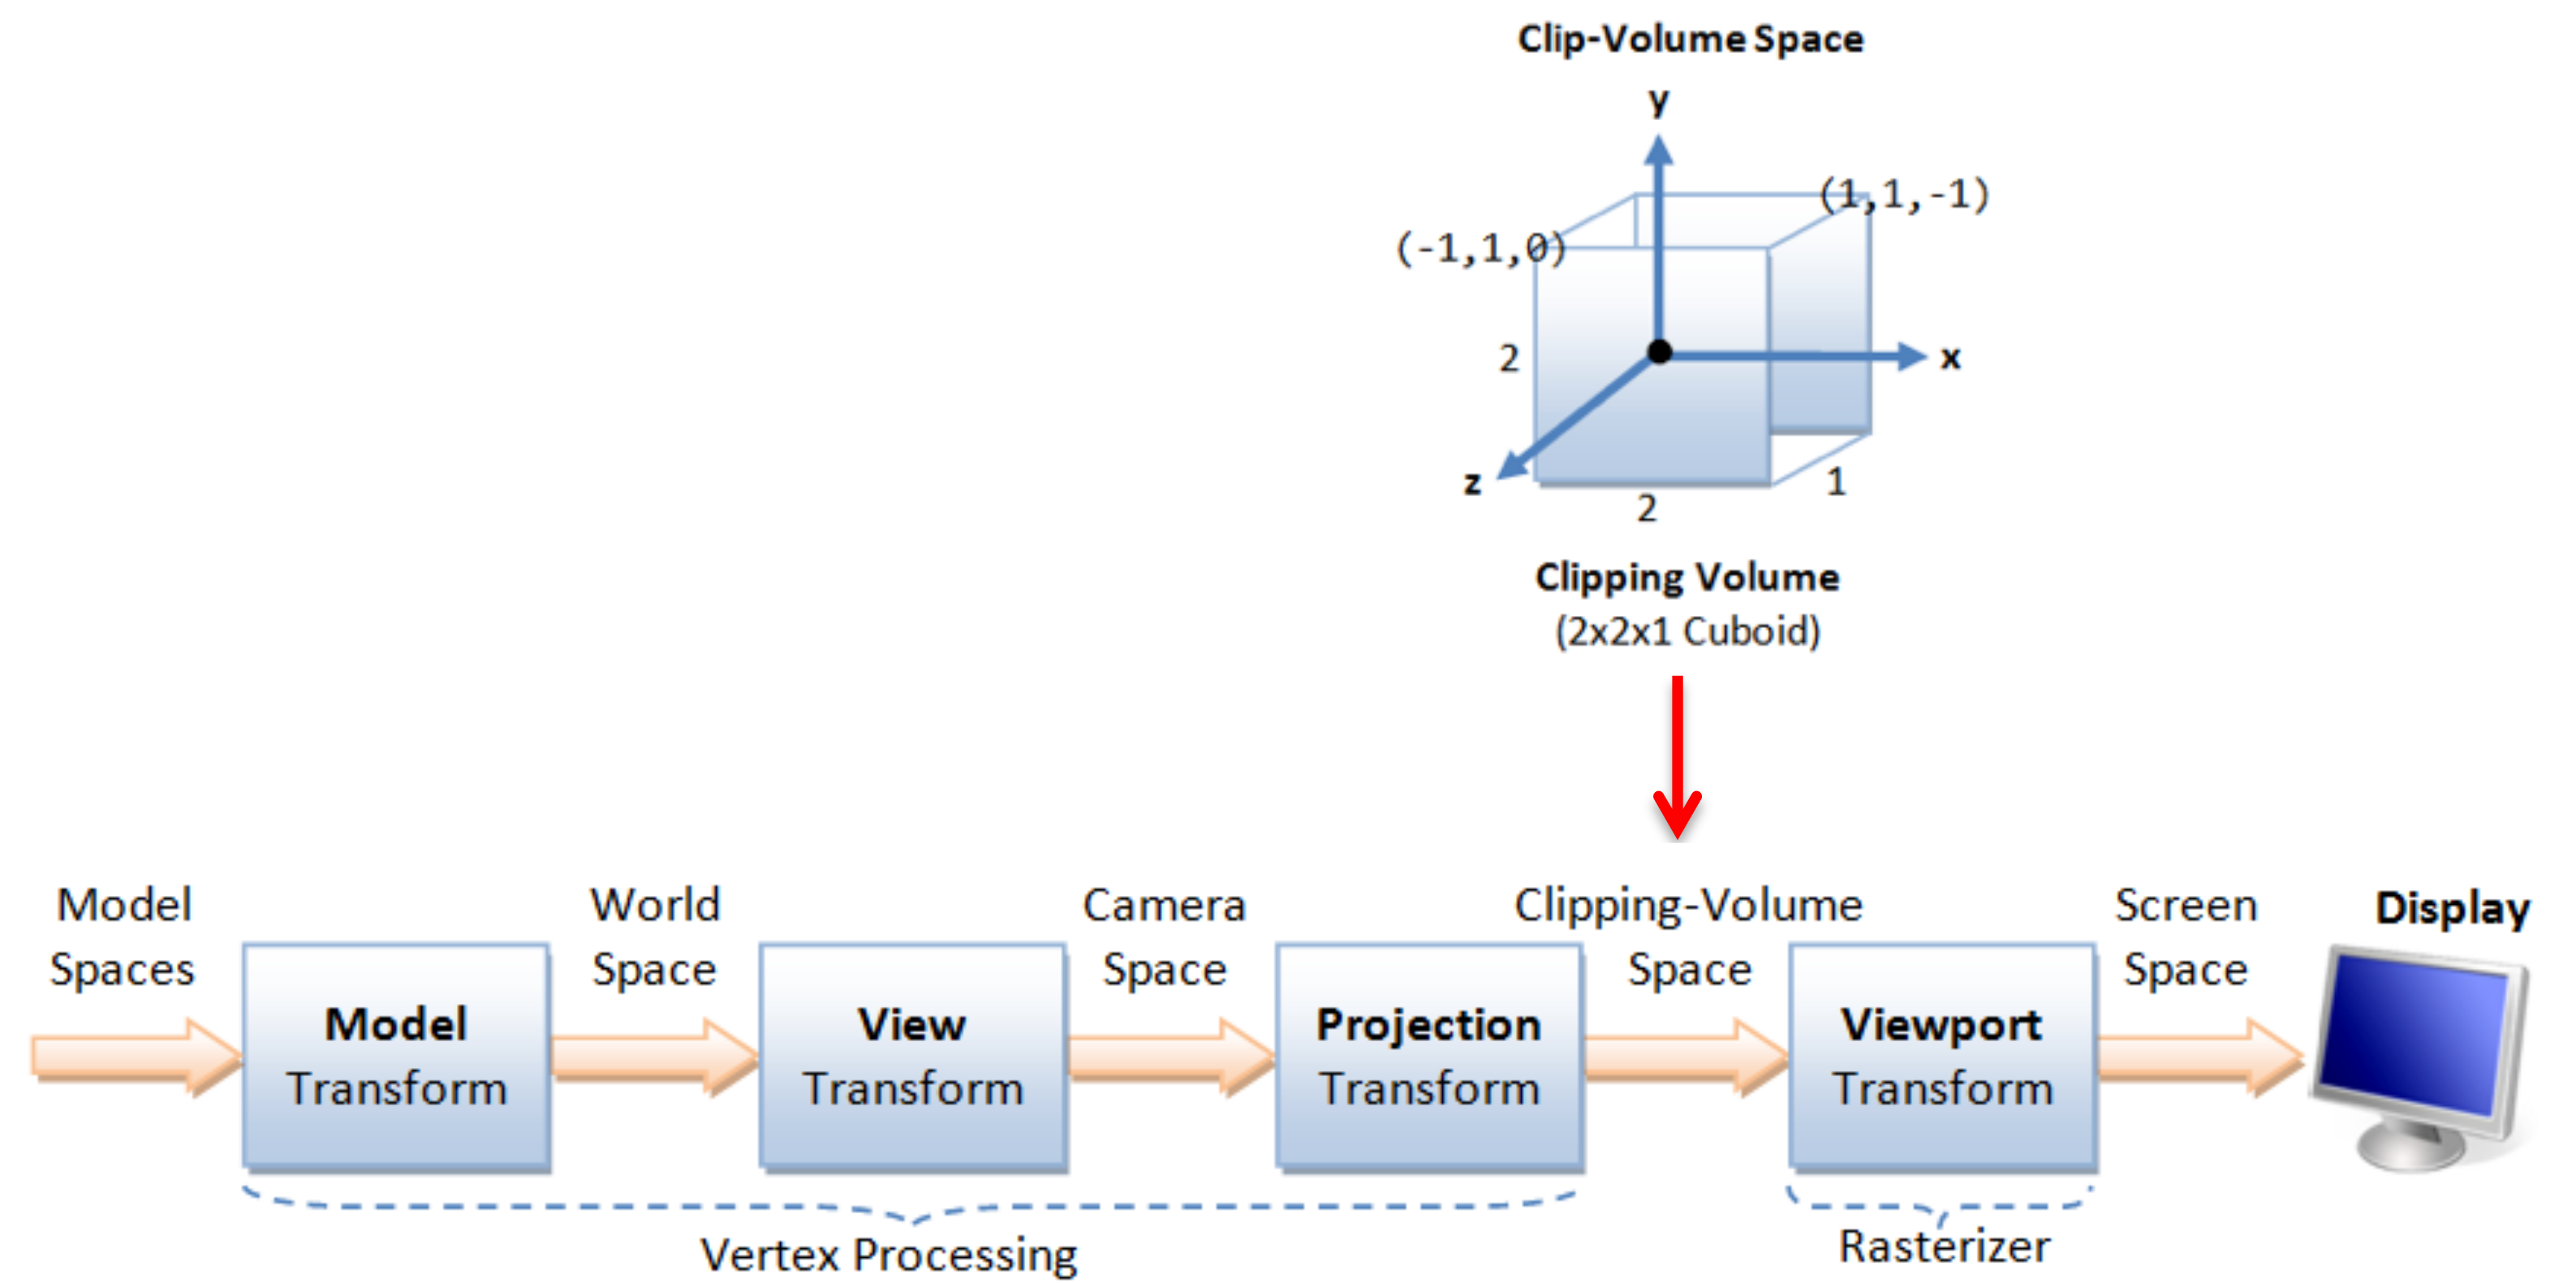
\includegraphics[width=10cm]{./slike/graphics_pipeline_04.png}
	\end{center}
\end{frame}

\begin{frame}{Protočni sustav i shaders}
	\begin{center}
		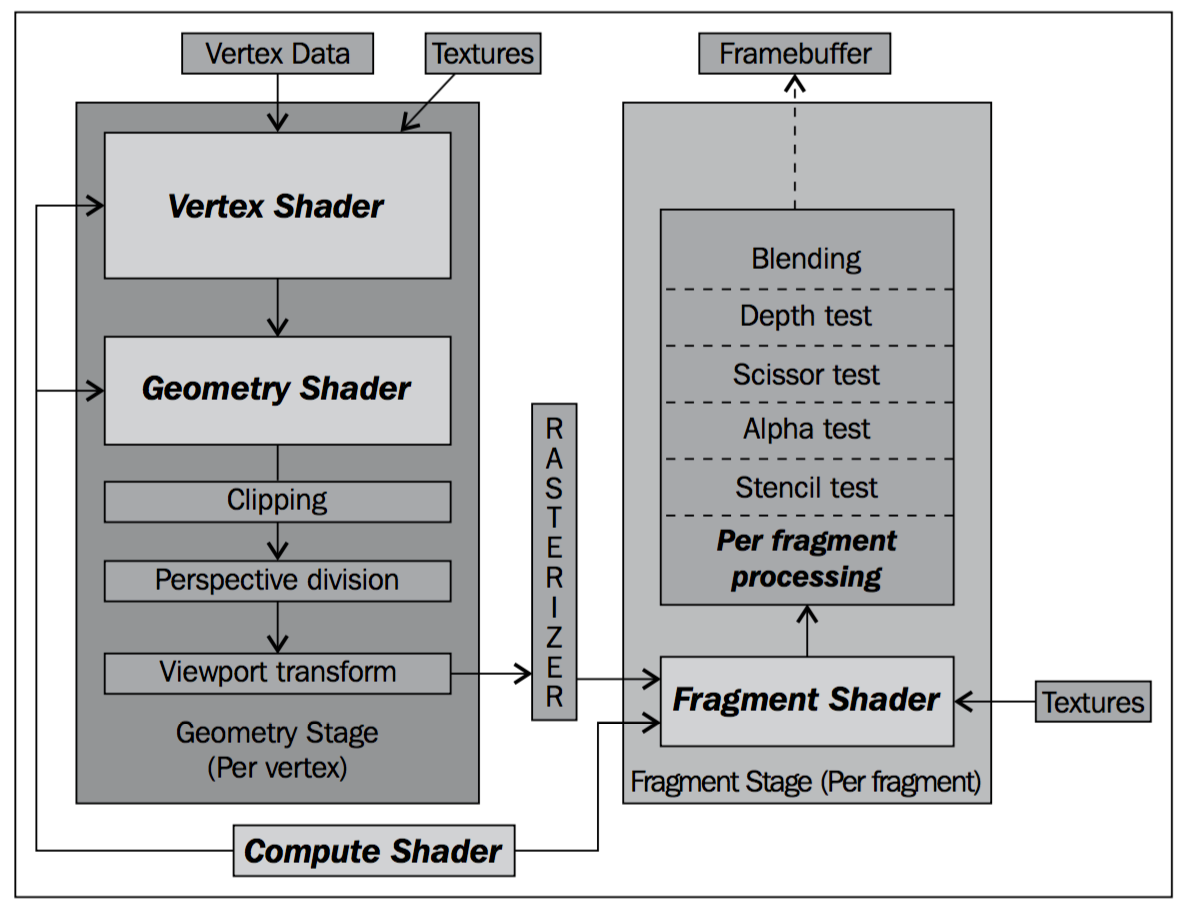
\includegraphics[width=8cm]{./slike/graphics_pipeline_05.png}
	\end{center}
\end{frame}

\section{Teksture}
\begin{frame}{Protočni sustav i teksture}
	\begin{center}
		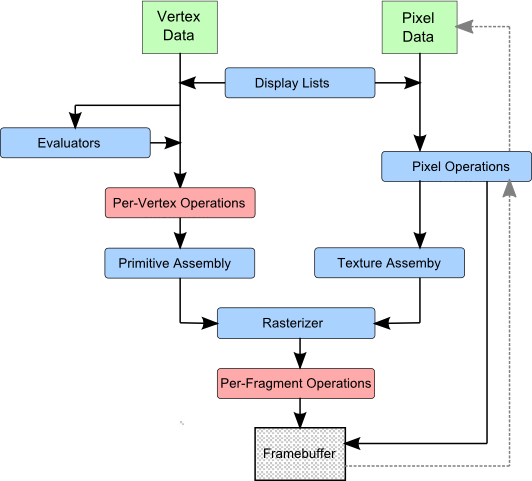
\includegraphics[width=8cm]{./slike/graphics_pipeline_06.png}
	\end{center}
\end{frame}

\begin{frame}{Teksture}
	\begin{center}
		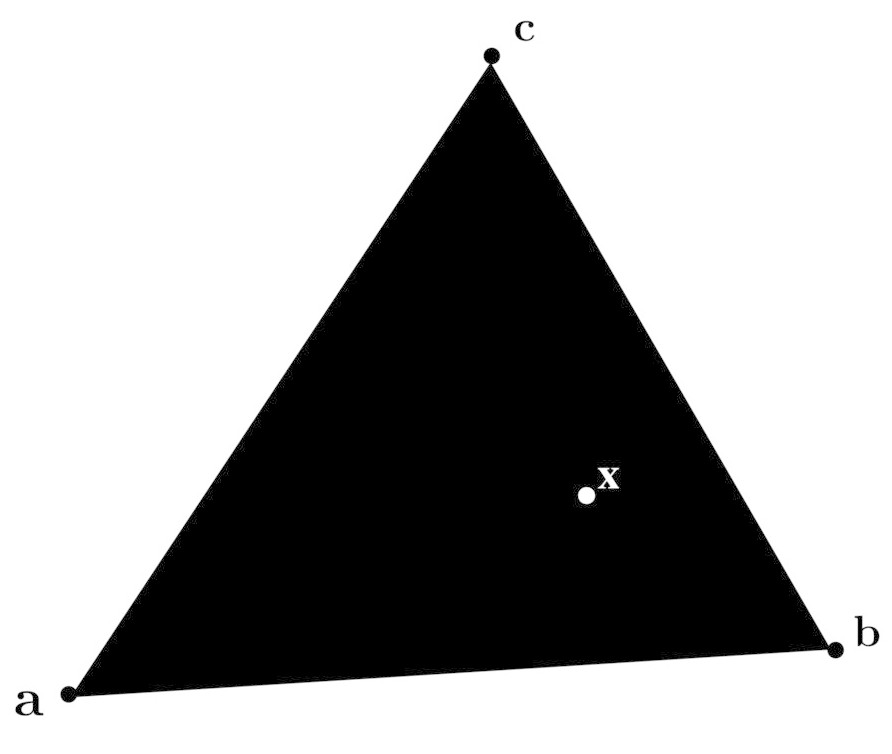
\includegraphics[width=6cm]{./slike/slide_023.jpg}
	\end{center}
\end{frame}

\begin{frame}{Teksture}
	\begin{center}
		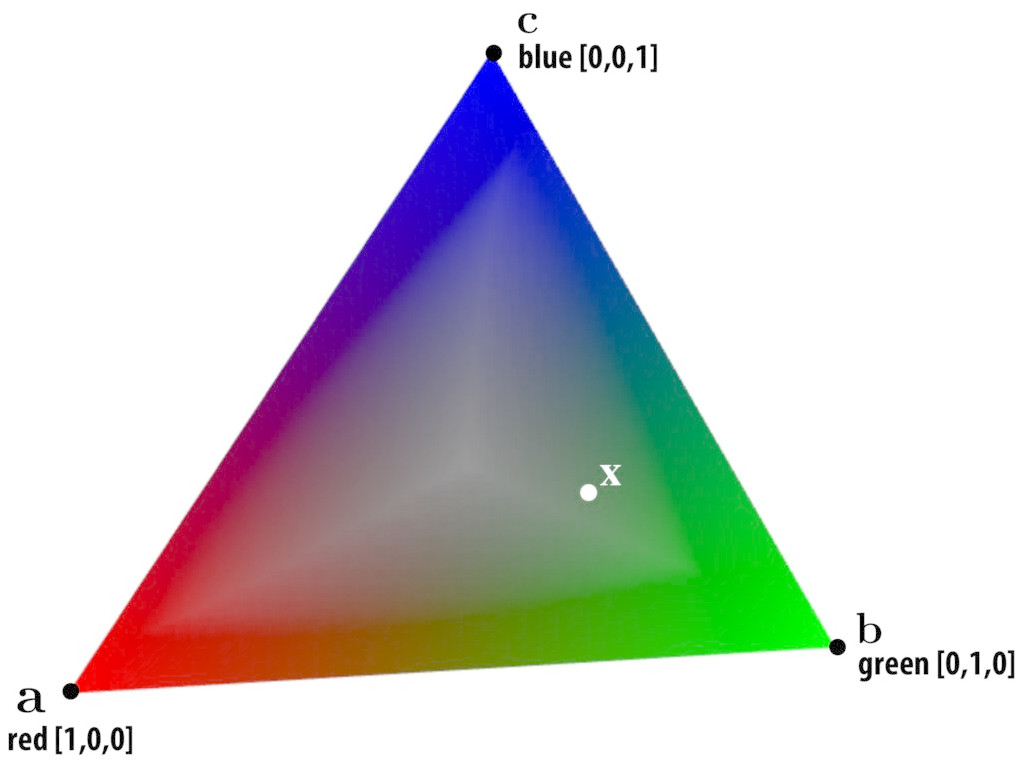
\includegraphics[width=6cm]{./slike/slide_024.jpg}
	\end{center}
\end{frame}


\begin{frame}{Teksture}
	\begin{center}
		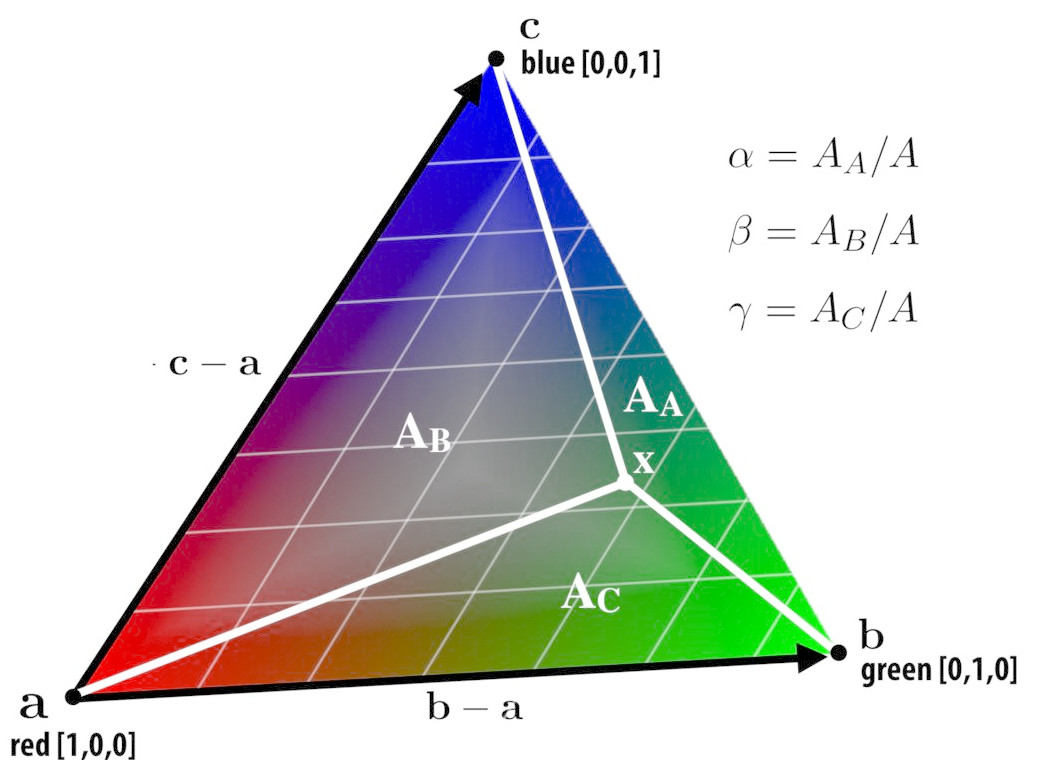
\includegraphics[width=6cm]{./slike/slide_029.jpg}
	\end{center}
\end{frame}

\begin{frame}{Teksture}
	\begin{block}{Algoritam}
		\texttt{for each covered screen sample (x,y):}\\
		\texttt{\ (u,v) = eval texcoord val at (x,y):}\\
		\texttt{\ float3 texcolor = texture.sample(u,v);} \\
	\end{block}
\end{frame}

\begin{frame}{Teksture}
	\begin{center}
		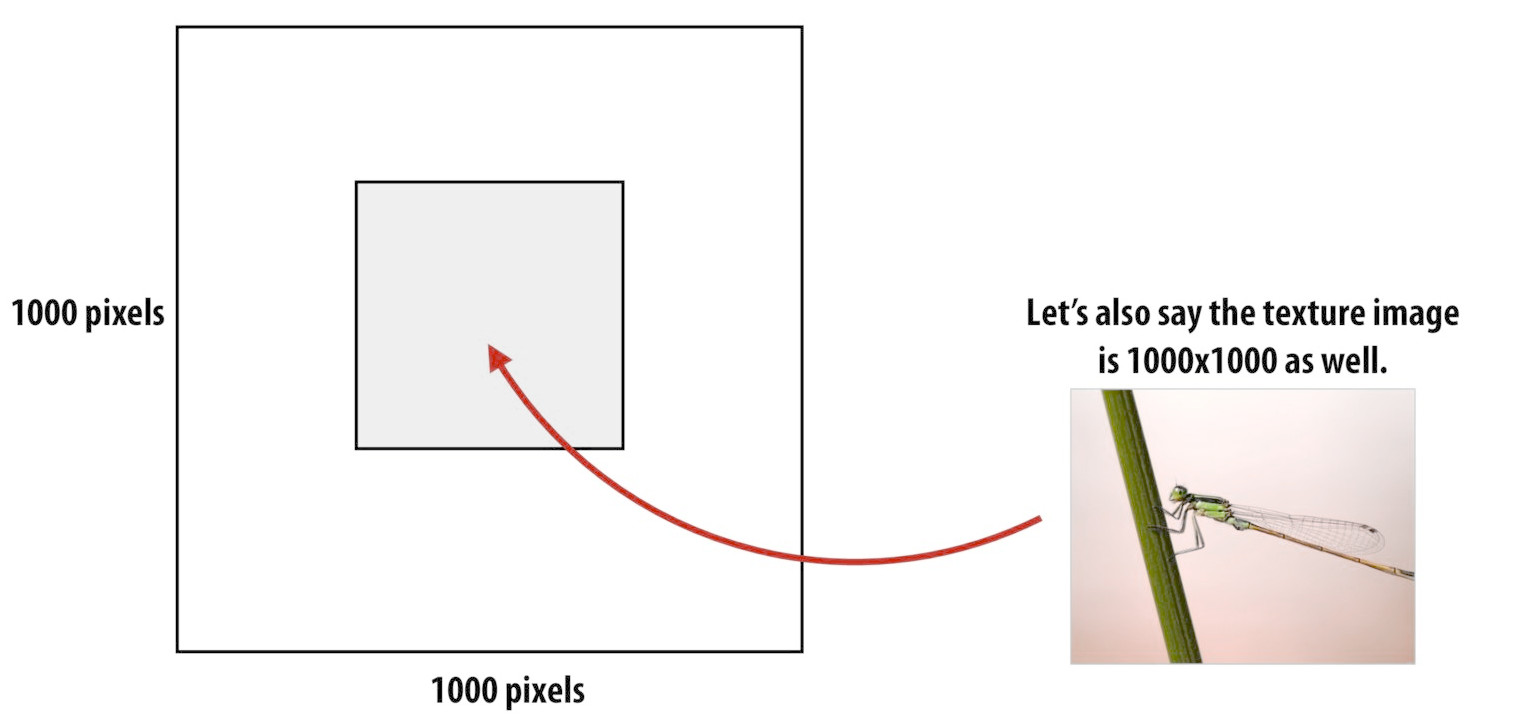
\includegraphics[width=6cm]{./slike/slide_050.jpg}
	\end{center}
\end{frame}

\begin{frame}{Teksture}
	\begin{center}
		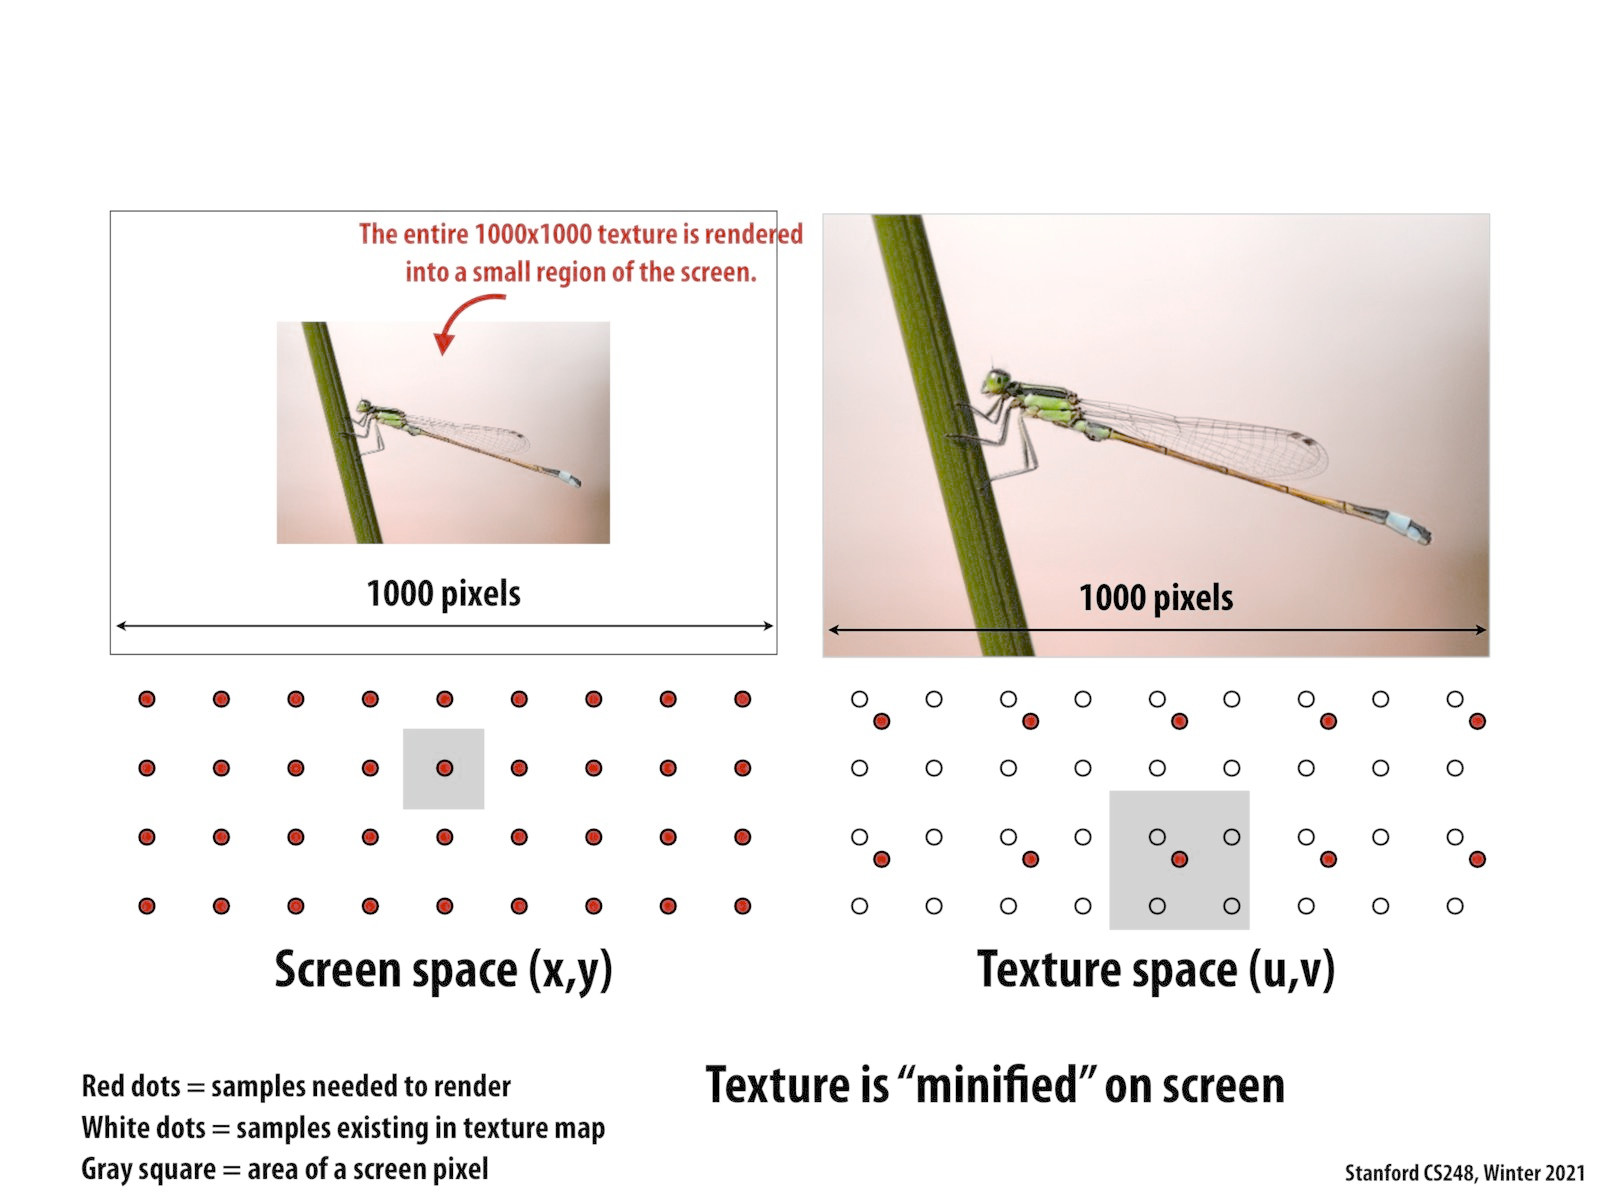
\includegraphics[width=6cm]{./slike/slide_051.jpg}
	\end{center}
\end{frame}

\begin{frame}{Teksture}
	\begin{center}
		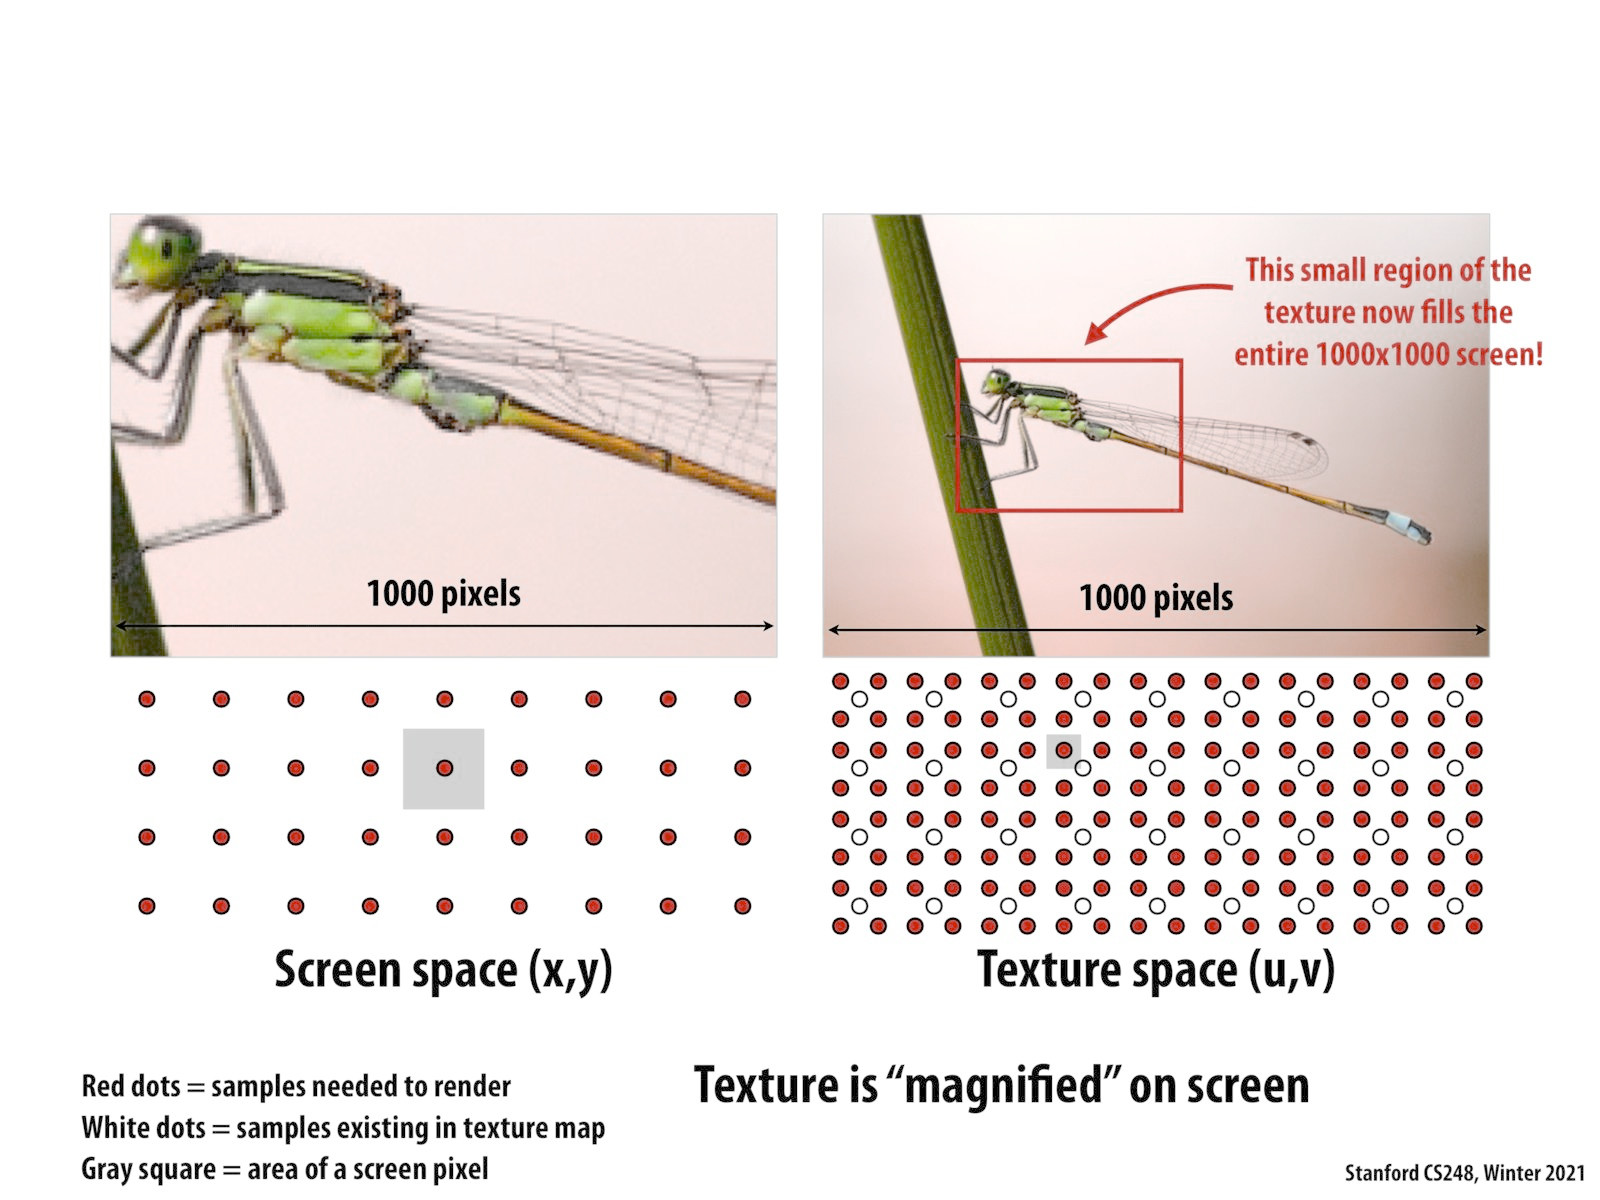
\includegraphics[width=6cm]{./slike/slide_052.jpg}
	\end{center}
\end{frame}

\begin{frame}{Teksture}
	\begin{center}
		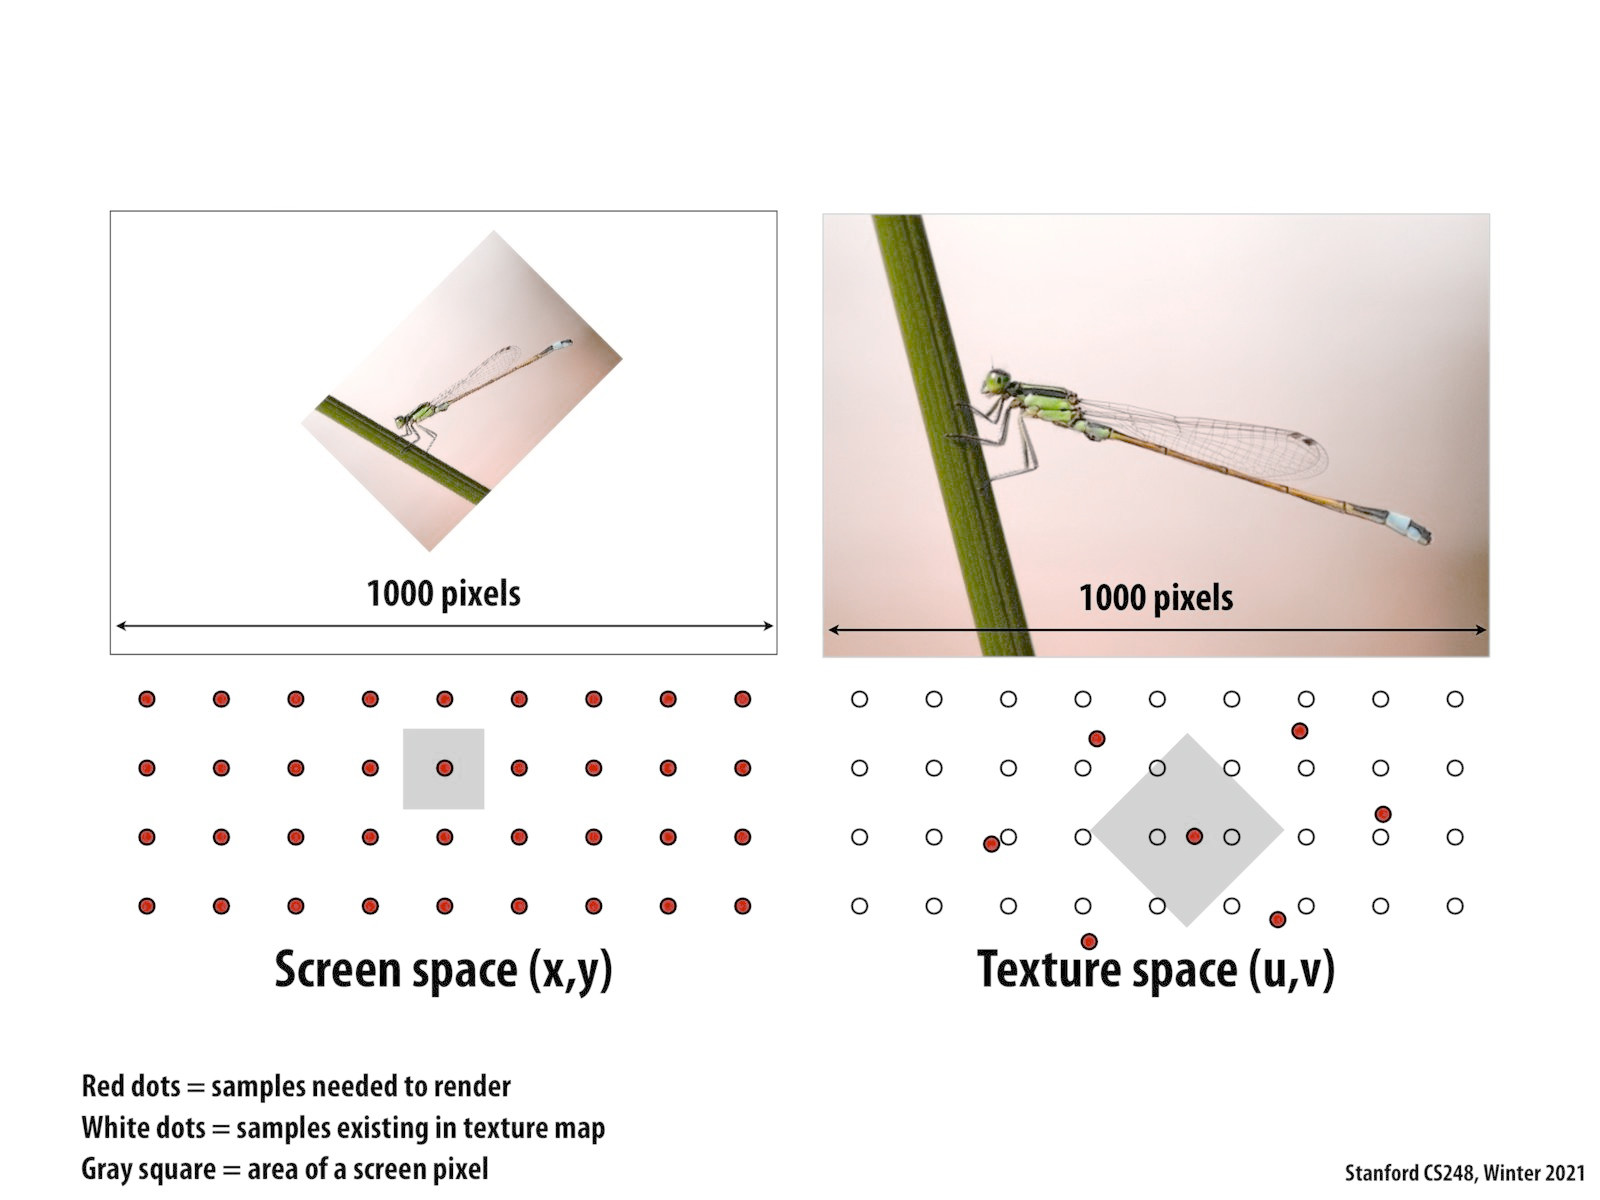
\includegraphics[width=6cm]{./slike/slide_053.jpg}
	\end{center}
\end{frame}

\begin{frame}{Teksture}
	\begin{center}
		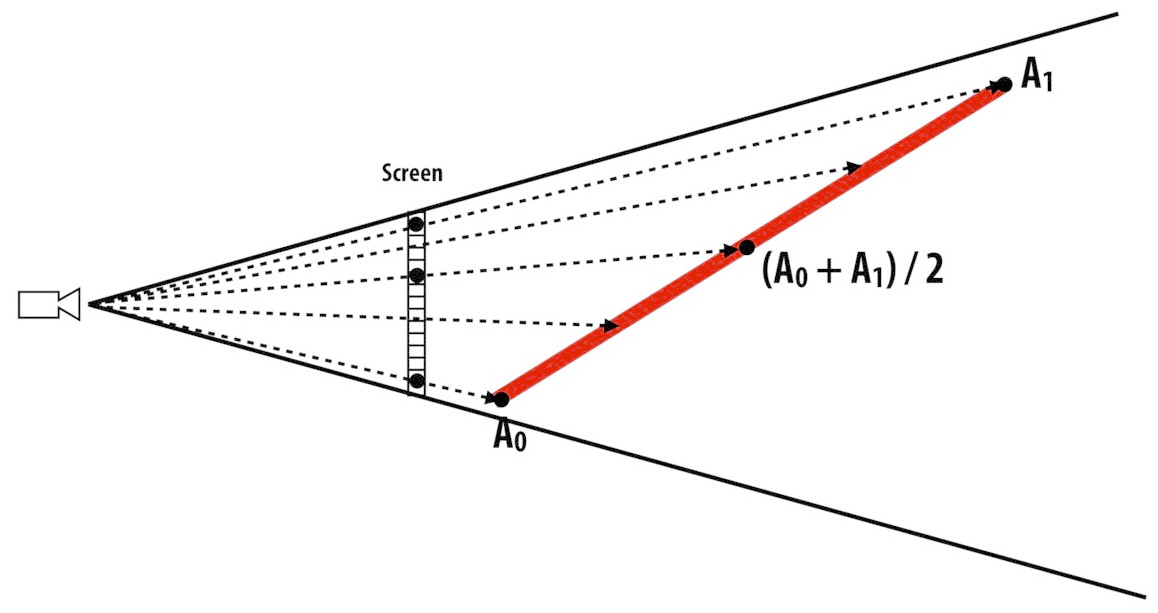
\includegraphics[width=6cm]{./slike/slide_030.jpg}
	\end{center}
\end{frame}

\begin{frame}{Teksture}
	\begin{center}
		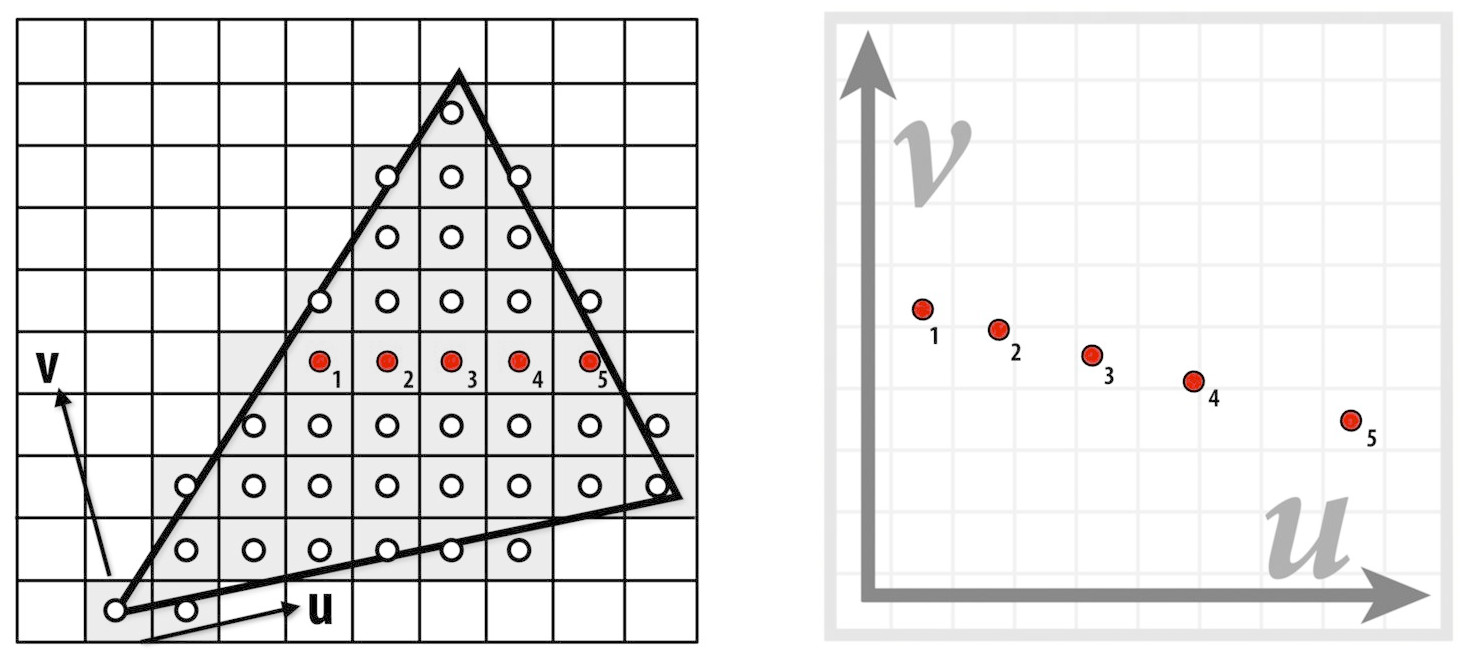
\includegraphics[width=6cm]{./slike/slide_054.jpg}
	\end{center}
\end{frame}

\begin{frame}{Posebne namjene}
	\begin{block}{Preslikavanje osvjetljenja}
		\begin{center}
			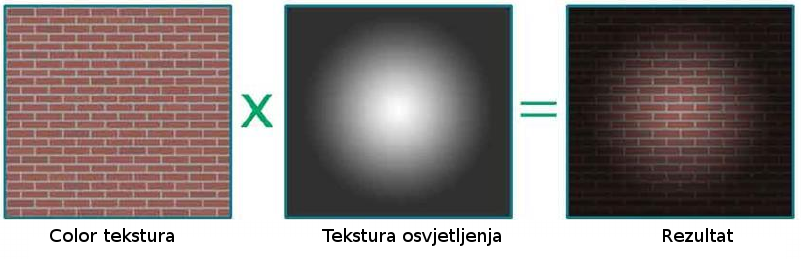
\includegraphics[width=6cm]{slike/teksture_light.png}
		\end{center}
		\begin{center}
			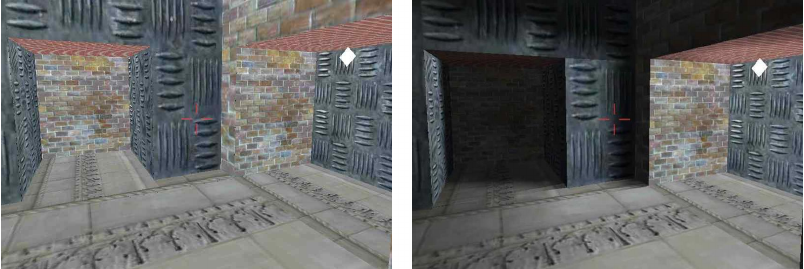
\includegraphics[width=6cm]{slike/teksture_light_02.png}
		\end{center}
	\end{block}
\end{frame}
%
\begin{frame}{Billboards}
	\begin{block}{Prozirne teksture}
		\begin{itemize}
			\item Preslikavanje teksture na poligon koji je uvijek okrenut prema promatraču (ili više
			statičnih poligona)
			\item Obično se koriste za prikaz drveća ($\alpha=0$ prozirno, $\alpha=1$ zeleno)
		\end{itemize}
	\end{block}
	\begin{center}
		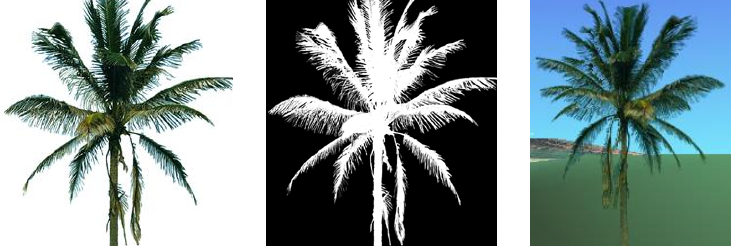
\includegraphics[width=6cm]{slike/teksture_billboards_01.png}
	\end{center}
	\begin{center}
		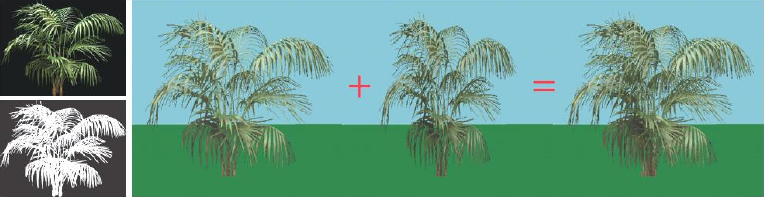
\includegraphics[width=6cm]{slike/teksture_billboards_02.png}
	\end{center}
\end{frame}
%
\begin{frame}{Posebne namjene}
	
	\begin{block}{Stapanje tekstura uz zadane prozirnosti - $\alpha$ blending}
		\begin{itemize}
			\item Više slojeva koji imaju definiranu prozirnost
			\item Konveksna kombinacija boja - $C = c_{a}\alpha_{a}+ c_{b}\alpha_{b}(1-\alpha{a})$ 
			\item prozirnost - $\alpha = \alpha_{a}+ \alpha_{b}(1-\alpha{a})$ 
		\end{itemize}
	\end{block}
	\begin{center}
		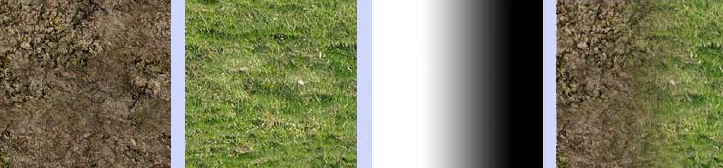
\includegraphics[width=9cm]{slike/07_prozirnost.png}
	\end{center}
\end{frame}

\plain{Pitanja?}
\end{document}